\chapter{Introduction}
An important field in astronomy and particle physics ever since Victor Hess discovered
the extraterrestrial origin of the atmospheric ionization
is astroparticle physics. Despite the rise
of terrestrial particle accelerators with ever higher beam energies,
the field is very relevant today. One of the reasons is that
even the biggest accelerators, like the LHC at CERN, got to a point where
increasing collision energies gets ever more difficult.

Even with all the previous achievements
there are still many questions about the structure of the universe, that we 
do not have an answer for yet.
Some of the prominent ones are:
\begin{itemize}
    \item{How does the space between galaxies look like? 
		Most of the known $\gamma$-ray sources are active galactic nuclei. 
		Knowing their properties allows to put constrains on
		intergalactic photon radiation and magnetic fields.}
    \item{Which particles form the dark matter and how do they interact? 
		It should be possible to detect dark matter annihilation by their emitted $\gamma$-rays.}
    \item{How exactly do relativistic outflows form in black holes?
		To this date the exact mechanism around the formation, structure and evolution of these
		jets is still unknown.}
    \item{By which processes and sources do cosmic rays get accelerated to the highest energies?
		The dtetails of the underlying processes are still unknown to the present date.}
\end{itemize}

Nowadays there exists a wide range of experiments trying to
answer these questions, not all focused on 
$\gamma$-ray physics.
In fact, they look at different particles and detection
mechanisms to detect
extraterrestrial particle sources, which is why
the term multi messenger astronomy is widely used.

\iffalse
In the following we will have a look at a brief overview 
of the emergence
of astroparticle physics and explain the key differences between 
the different observable messenger particles.
We will then focus at the 
most influential IACT experiments to motivate the construction of 
the Cherenkov Telescope Array.
\fi

\section{The Origins of Astroparticle Physics}
In 1909 Theodor Wulff measured the radiation on top of the 
Eiffel tower in Paris
\cite{horandel2013early}.
Assuming that most radiation came from the 
earth crust, the decrease was less than expected.

Several balloon flights 
of different physicists (for a contemporary overview of the field see e.g. \cite{luftelektrizitaet})
and underwater experiments of Domenico Pacini in 1910 
\cite{2011arXiv1101.3015P}
lead to the conclusion that most of the radiation must indeed be
of extraterrestrial origin, which was not immediately accepted 
in the community though \cite{bookap}.

Evidence came with the extended balloon flights of Victor Hess
\cite{Hess:1912srp}:
Not only was the intensity decrease with higher altitude not 
matching the expectations, but at a certain point at around 
\SI{2000}{\meter} the intensity 
was actually increasing again.
As this was also the case in night flights, the sun
was excluded as possible source.
A few years later, in 1929, Werner Kolhörster and 
Walther Bothe confirmed these experimental results \cite{bothe1929wesen}.

The radiation was referenced as "Höhenstrahlung" 
(see e.g. \cite{myssowsky1926versuche}) 
and "cosmic rays" (see e.g. \cite{millikan1928origin}) with 
the english term cosmic rays eventually winning out.

Experiments of Jacob Clay in 1927 
\cite{clay1927penetrating}
lead to the further insight that the main proportion of 
the radiation must carry an electric charge.

With experiments resolving around the influence of the earth magnetic 
field by 
Bruno Rossi \cite{Rossi1933},
Thomas H. Johnson \cite{PhysRev.43.834},
Luis Alvarez and Arthur H. Compton \cite{PhysRev.43.835}
in 1933,
a positive charge was conducted.

The remaining puzzles towards astroparticle and $\gamma$-ray
astronomy were solved with the discovery of antimatter in a cloud chamber
by Carl D. Anderson in 1933 \cite{PhysRev.43.491}
and the discovery of air showers by detecting coincident 
events in separated Geiger-müller tubes by 
Bruno Rossi in 1934
\cite{PhysRev.45.212}
and their later description by
the team around Pierre Auger 
\cite{RevModPhys.11.288}.

In the following years multiple particles with direct use in the 
astrophysics have been found:
The pions \cite{LATTES1947}, the muons \cite{PhysRev.52.1003}
and the neutrinos \cite{Cowan103}.

Recently the so far last discovery on this journey
was made with the measurement of the first gravitational 
waves \cite{PhysRevLett.118.221101}.

\section{Multimessenger astronomy}

Nowadays we observe extraterrestrial processes on four channels: 
\begin{enumerate}
	\item Electromagnetic radiation
	\item (Charged) cosmic rays
	\item Neutrino radiation
	\item Gravitational waves
\end{enumerate}

All of the accompanying particles have vastly different
properties and require different experimental setups.
A common thing is to observe the same sources 
on different channels to learn more about the processes that happen at 
these far distant sources. This is what is often times 
referred to as multi messenger astronomy (see e.g. \cite{RevModPhys.85.1401}, where
measurements of neutrinos and gravitational waves get combined).
Figure \ref{fig:multi_messenger} illustrates the key differences between
photons, protons and neutrinos.

Before we focus on the special field of IACTs, we will have
a brief look at the different messenger particles.

\begin{figure}
	\centering
	\captionsetup{width=0.9\linewidth}
	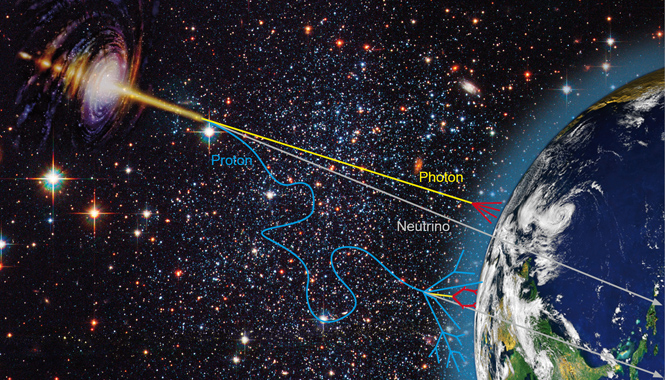
\includegraphics[width=0.9\textwidth]{images/astro-web-titel.jpg}
	\caption{Visualization of the behaviors of different messengers
		particles in modern astronomy.
		Photons and neutrinos travel the universe without deflection,
		because they do not carry an electric charge.
		Neutrinos interact less than photons both in the universe and in the detector,
		which leads to a high proportion passing through earth.
		Charged cosmic rays get deflected by interstellar
		magnetic fields and thus generally do not allow for a assignment to a cosmological source.
		This illustration lacks gravitational waves 
		as these have only recently been measured.
		The image is taken from the DESY-website at \cite{desy_mm_astro}.
	}
	\label{fig:multi_messenger}
\end{figure}


\subsection{Gamma Rays}
In contrast to charged cosmic rays, $\gamma$-particles point towards
their sources, allowing to search for sources of radiation.
In general $\gamma$-radiation refers to photons at all wavelength,
the term $\gamma$-rays in contrast is assigned to the very 
highest energy particles with energies above those of X-rays.
A schematic illustration of the different photon wavelengths
can be seen in figure \ref{fig:em_spectrum}.

\begin{figure}
	\centering
	\captionsetup{width=0.9\linewidth}
	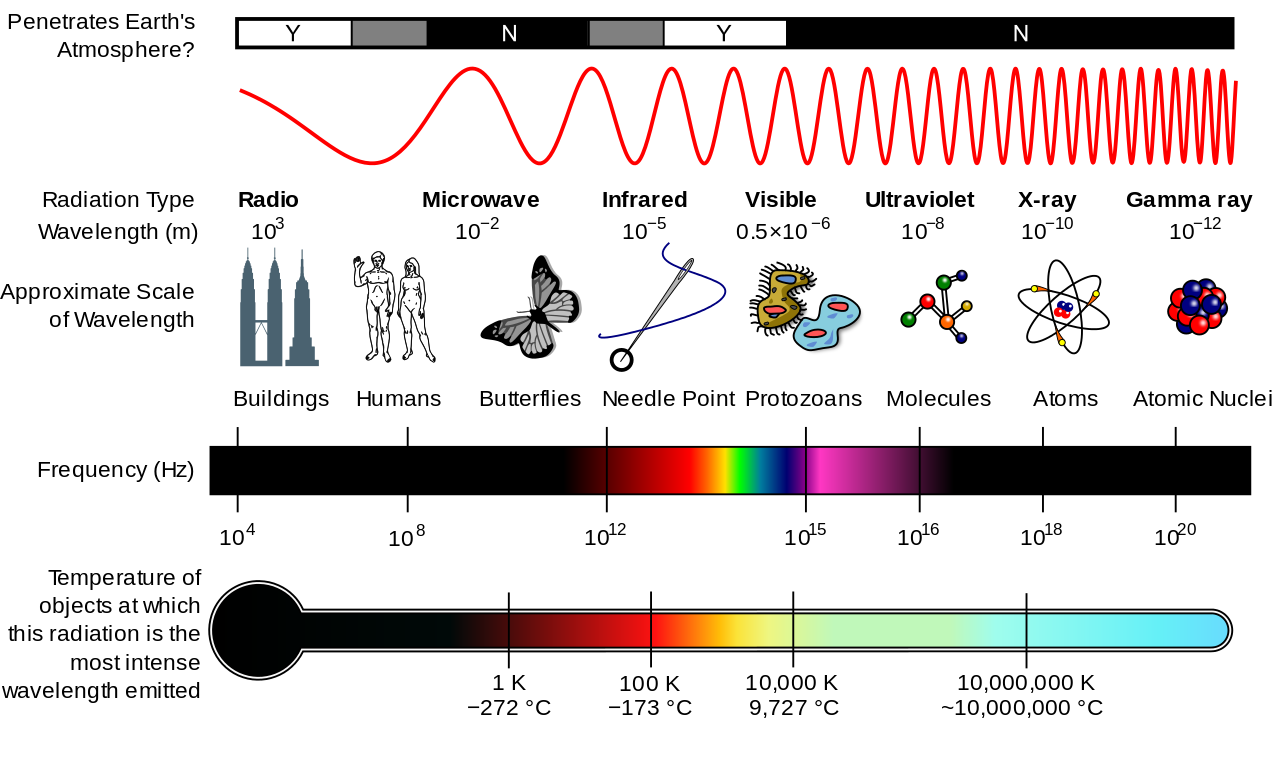
\includegraphics[width=.9\textwidth]{images/em_spectrum.png}
	\caption{An overview of properties and applications of photons
		on a wide range of wavelengths.
		Radio-photons possess very low energies, gamma-rays 
		carry the very highest energies.
		Visible light lies in between, technical 
		applications exist for all the shown wavelengths.
		As indicated by the temperature bar at the bottom,
		$\gamma$-rays can not feasibly be produced by thermal radiation.
		The image is taken from \cite{wiki_em}.}
	\label{fig:em_spectrum}
\end{figure}

Creation of high-energy gamma-rays is due to a lot of 
different processes. Among these we want to give a brief 
overview of two important processes, focusing on 
photon emission from an initial pure electron distribution.
Depending on the studied case other emission factors 
might play important roles as well, such as 
the $\gamma$-production from $\pi^0$-decays in cosmic rays.

\textbf{Synchroton Radiation}

Sources of cosmic and gamma rays often times include 
high magnetic fields. Any moving charged particle will thus be
deflected perpendicular to its moving direction
due to the Lorentz-force, forcing them on a radial trajectory.
At the same time a relativistic charged particle, 
that gets accelerated radially, emits synchroton 
photons with average energy given by 
equation \ref{eq:synchroton}

\begin{equation}
	\langle E_{\gamma} \rangle \propto \frac{1}{M_P} E_P^2 B^2.
	\label{eq:synchroton}
\end{equation}

Hereby $M_P$ and $E_P$ denote the accelerated particle's 
mass and energy respectively. With the inverse mass dependency 
it is immediately evident that 
synchroton radiation plays a major role in leptonic 
emission and much less in hadronic emission.

It is important to remember that this affects the 
initial electron distribution, by reducing the electrons energy.
This is sometimes referred to as synchroton cooling.

The emitted synchroton spectrum needs to be further modified 
if the emitting region is optically thick and photons 
get absorbed by the medium.
This is always true for our cases, as the regions contains 
both magnetic fields and a high density of electrons.

\textbf{(Inverse) Compton Scattering}
In a classical particle interpretation photons and electrons 
can collide exchanging energy and altering their directions.
For the normal case of Compton scattering the electron 
is assumed to be at rest and the photon can never gain 
energy by scattering of the electron.
This can be 
seen by the increase in wavelength in equation \ref{eq:compton},
with $\lambda^{\prime}$ denoting the the scattered photons 
wavelength, $\lambda$ denoting the initial photons wavelength  
and $\Theta$ the scattering angle.

\begin{equation}
	\lambda^{\prime} - \lambda  \propto \left(1-\cos{\Theta} \right)
	\label{eq:compton}
\end{equation}


If the electron itself is moving with much higher energy
than the photon, this changes and the photon can gain substantial energy.
This is referenced as inverse Compton scattering.
In that case transforming the equations to the 
electron's frame of reference and back to the labor frame 
boosts the photons energy by a factor $\gamma$ for each transformation, 
with $\gamma$ being the Lorentz factor of the electron.

A limit to the photon energies is set by the scattering cross
section, which reduces with higher photon energies.
For low energies the cross section can be approximated by 
the Thomson cross section, for high energies
one uses the Klein-Nishina cross section.

The Synchroton Self Compton model combines the above mentioned
effects to produce a photon energy distribution from an
electron distribution, which is often times assumed to
follow a power-law spectrum initially.
The free parameters of the model can be interpreted as 
three frequencies: The minimum injection frequency $\nu_m$, 
the cooling frequency $\nu_c$ and the self-absorption frequency $\nu_a$.
Depending on the order of these parameters, different 
photon distributions can be generated.

For more general information about the generation of photon 
and cosmic ray spectra, the reader is referred to 
\cite{gaisser_engel_resconi_2016}
or
\cite{bookap}.

For a detailed analysis of the influence of the parameters of
the Synchroton Self Compton model, 
the lecture of \cite{10.1093/mnras/stt1461} is advised.


Emitted $\gamma$-rays can be observed either directly
from outside the atmosphere via satellites or indirectly
via ground based gamma astronomy. In the later case
IACTs are used to detect electromagnetic showers induced
by the collision of high energy photons with particles in the atmosphere.
% An example for direct observation could be the Fermi 
% Gamma-Ray Space Telescope \cite{Atwood_2009},
% an example for ground based observation could be the
% MAGIC-experiment \cite{LORENZ2004339}.

\subsection{Cosmic rays als background erwähnen}


\iffalse
\subsection{Neutrinos}
Even less affected by interactions on the way 
from the source to the earth are neutrinos ($\nu$).
Due to their small interaction cross sections and no electric charge, they 
suffer very little from absorption or deflection.
For very much the same reasons detecting neutrinos is much harder
than detecting photons or charged particles.

The small cross section requires to build huge detectors, 
the ICECUBE having a detector volume of \SI{1}{\kilo\meter^3}
\cite{Abbasi:2008aa}.
An illustration of the ICECUBE Neutrino Observatory
is shown in figure \ref{fig:icecube}.
\begin{figure}
	\centering
	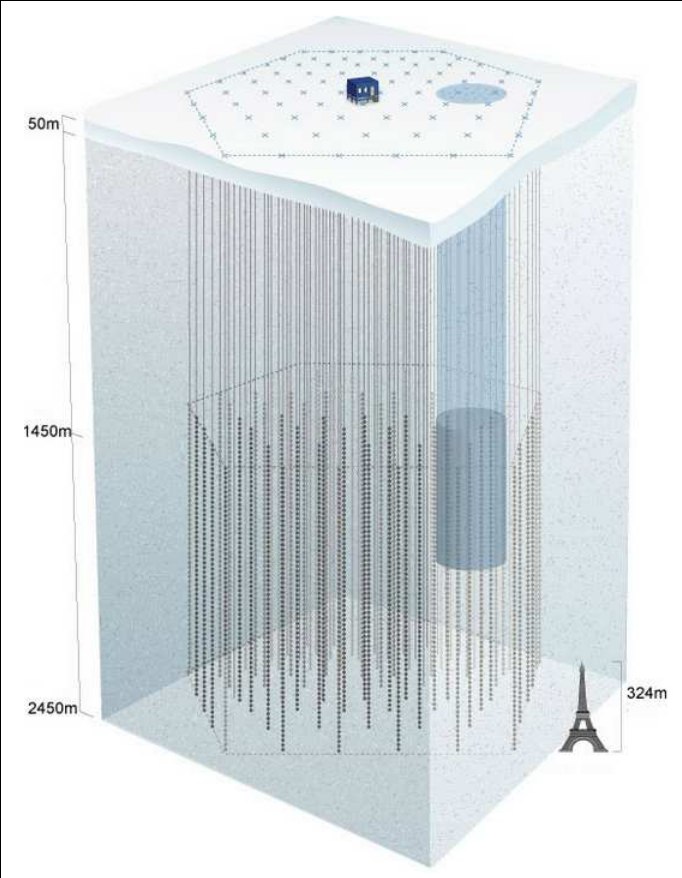
\includegraphics[width=0.8\textwidth]{images/icecube.png}
	\caption{icecube illustration, cite that \cite{Abbasi:2008aa}}
	\label{fig:icecube}
\endrvation.
They are a direct result from general relativity and occur
at certain constellations of very high masses, such as 
merging black holes.

An illustration of such an event is shown in figure \ref{fig:gravi_waves}. 
\begin{figure}
	\centering
	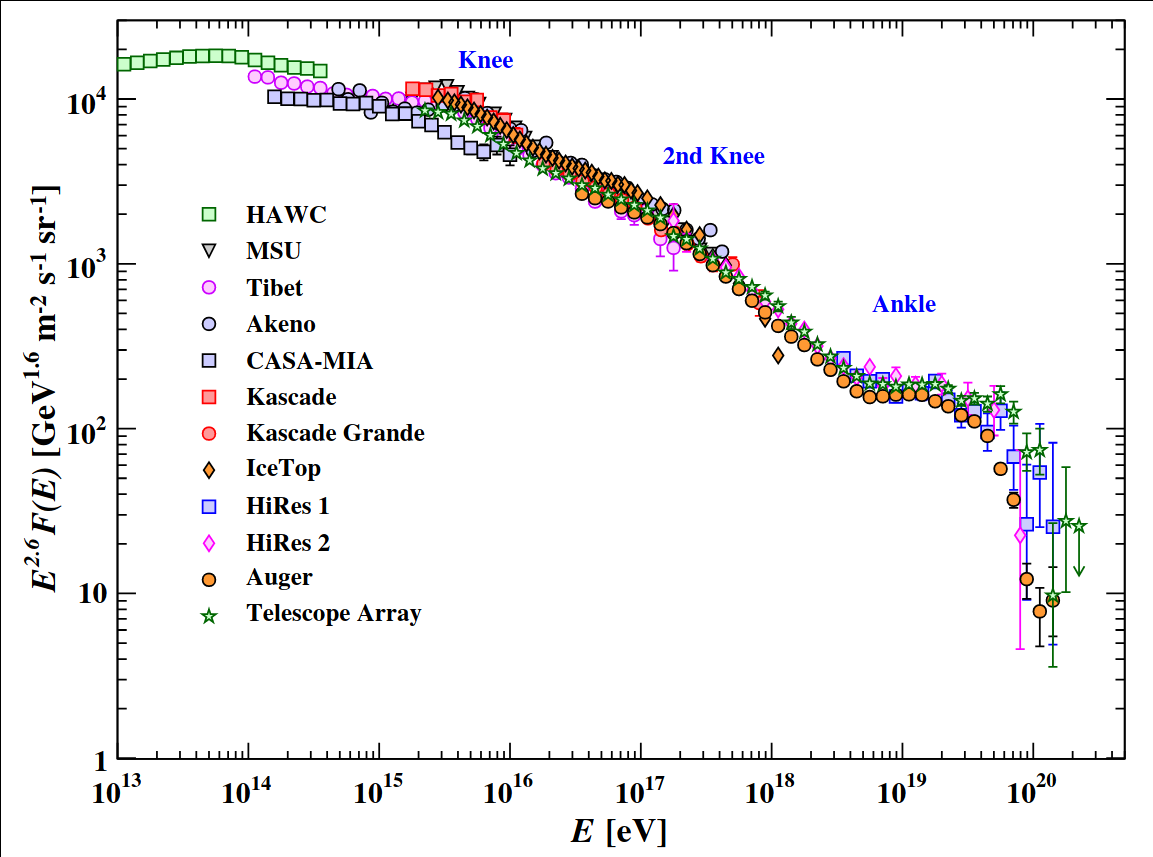
\includegraphics[width=0.8\textwidth]{images/cr_spectrum.png}
	\caption{images}
	\label{fig:gravi_waves}
\end{figure}


We can detect them using large size interferometers such as
the LiGO's three detectors (citation needed).
\fi



\section{Detection of Gamma Rays}

\subsection{Andere Methoiden, warum iacts?}
\subsection{Kram drunter als IACT}
The primary particles of gamma or cosmic rays cannot be 
observed with IACTs directly. Instead one can measure the secondary particles
that emerge from the particles interaction with matter.

If the primary particle energy is high enough, the resulting 
secondary
particles can interact with the atmosphere themself, thus starting a 
cascade of secondary particles.

Depending on whether the primary particle is 
a photon/electron/positron or a heavier particle such as a proton 
or iron core, the interactions vary.

This leads to a separation of electromagnetic and hadronic showers.
If the experiment is primarly looking for 
gamma rays, e.g. if measuring a known source like the Crab Nebula, 
the hadronic showers act as dominant background.
As hadronic showers get observed much more frequently, 
the identification of the primary particle type is a very important 
task, often times referred to as gamma-/hadron-separation.

To understand how these showers differ, we will have a very brief look
at the relevant interactions at the primary particle energies
we want to observe.

\subsection{Electromagnetic Showers}
Electromagnetic showers consist mainly of three types of particles:
\begin{enumerate}
	\item{Photons $\gamma$}
	\item{Electrons $e^-$}
	\item{Positrons $e^+$}
\end{enumerate}

The main interaction for high energy photons is pair 
production, generating an $e^+/e^--$pair where the energy of 
the secondary particles equals the photon energy.
On the other hand high energy electrons (and positrons) lose 
most of their energy by radiation, leading to a photon with 
an energy close to the electron energy.
Only at lower particle energies other interaction forms show their impact,
with particle scattering and ionization 
leading to more continuous energy losses.

These assumptions lead to the most basic model of an 
electromagnetic shower, proposed by Bhabha and Heitler in 1937
\cite{doi:10.1098/rspa.1937.0082}.
It starts with a high energy primary photon before its interaction in the atmosphere 
(The original paper starts from a high energy electron interacting in lead actually.
As will be evident this does not concern our qualitative look at the model.) and continues 
the calculation in discrete epochs.
The photon produces a pair of $e^-$ and $e^+$ in the first epoch.
Because of the high energies at play, the direction of these secondary 
particles does not deviate significantly from the photons direction, 
making the problem essentially one-dimensional.
The $e^+/e^-$ continue on to radiate a photon each and the cycle continues.
Each step doubles the number of particles in the shower with each particle 
on average getting half the energy of its parent particle.
These processes continue until the energy of the $e^+/e^-$ becomes low enough for
continuous ionization processes to become relevant.
At this point the particle is considered to be stopped and the shower
does not evolve further.

Today Monte Carlo calculations get used to simulate the properties 
of particle showers in the atmosphere.
The most common software to model the atmospheric interactions is
CORSIKA \cite{Engel:2018akg}.

Figure \ref{fig:gamma_shower} illustrates the Bhabha-Heitler model (left)
and a \SI{100}{\giga\electronvolt} gamma shower, simulated with CORSIKA (right).

\begin{figure}
	\centering
	\captionsetup{width=0.9\linewidth}
	\begin{subfigure}{.7\textwidth}
  		\centering
  		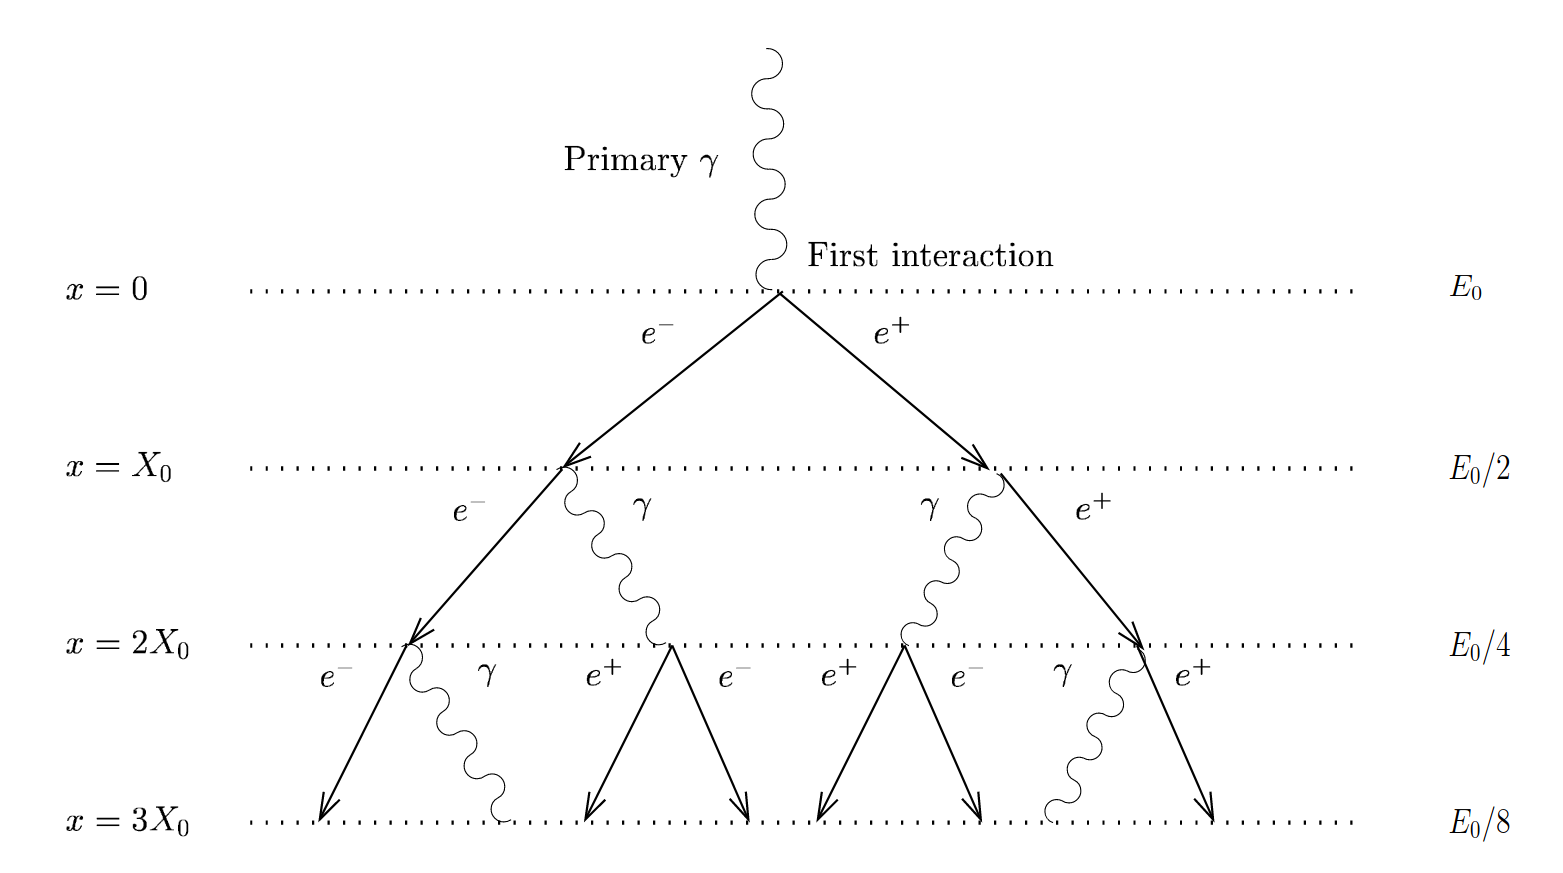
\includegraphics[width=\linewidth]{images/em_shower_illustration.png}
	\end{subfigure}%
	\begin{subfigure}{.2\textwidth}
 		\centering
		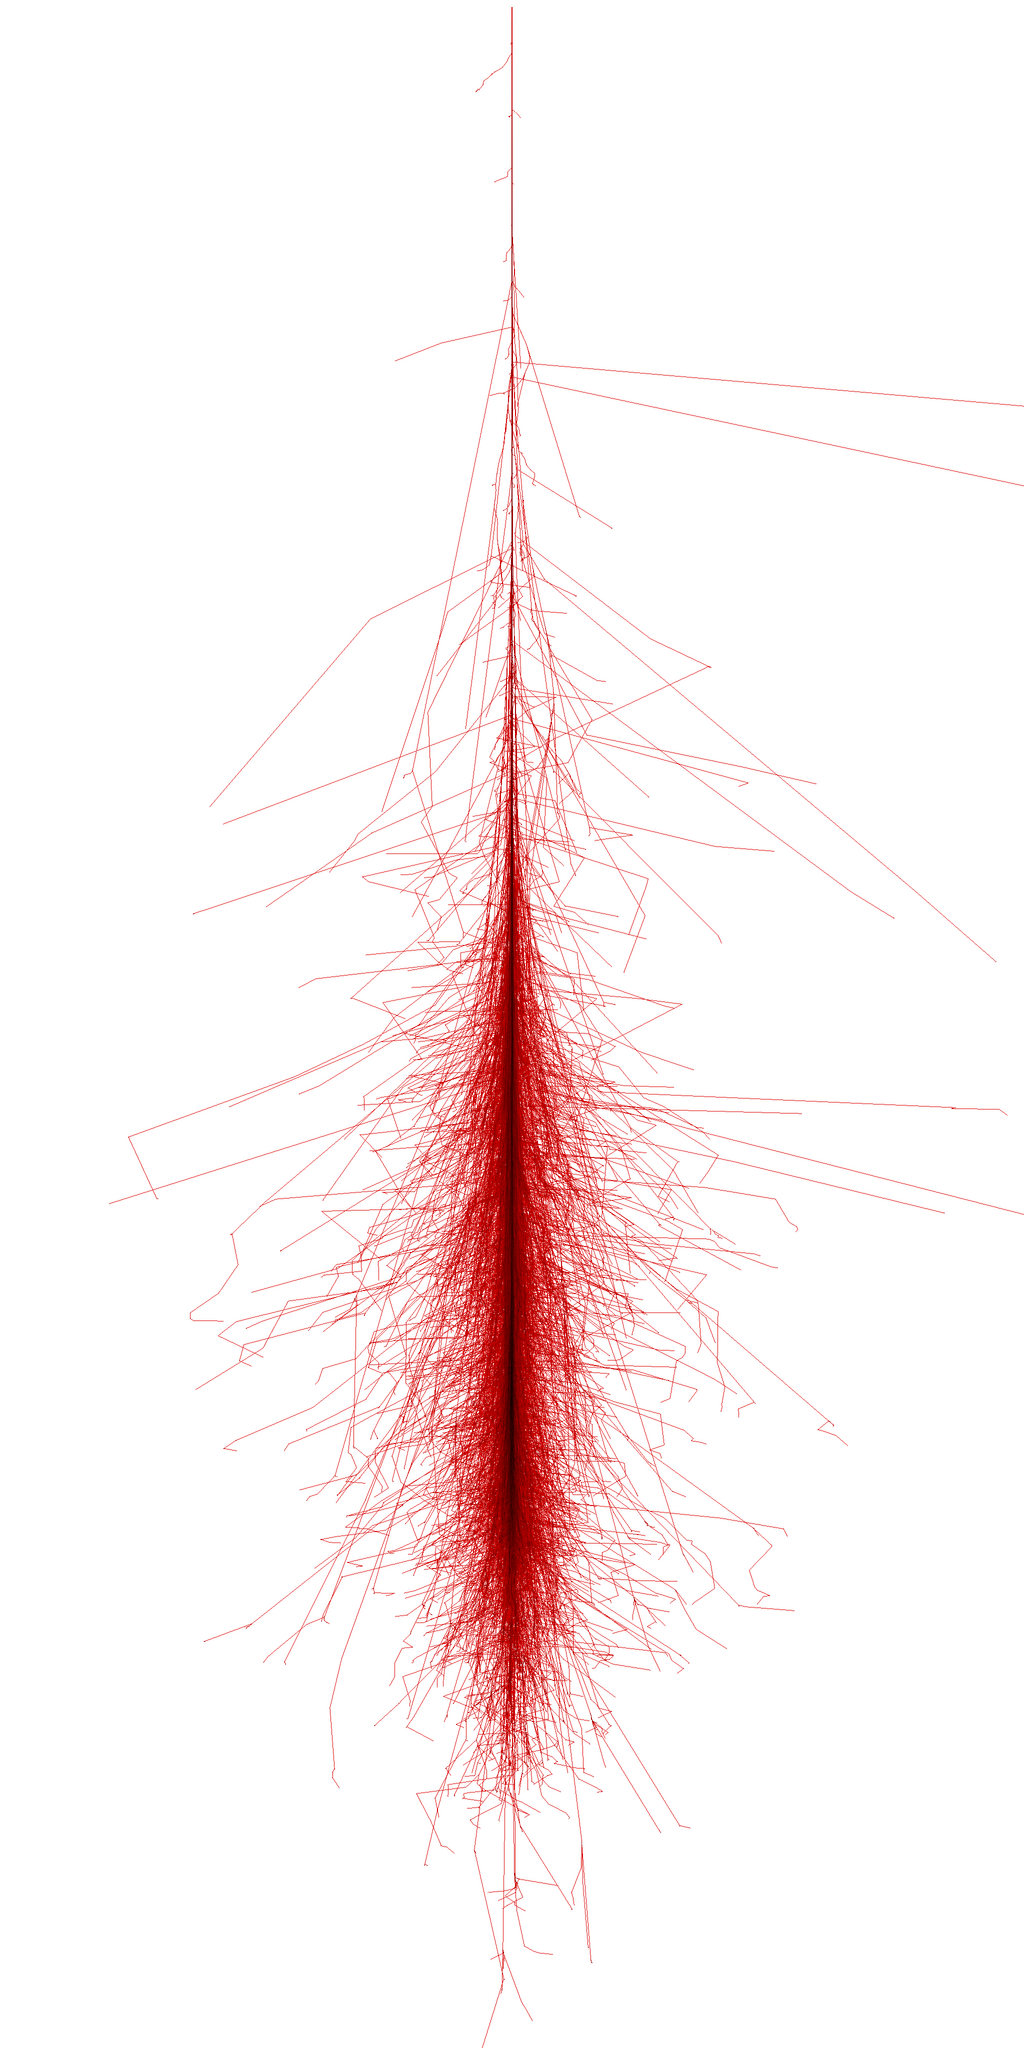
\includegraphics[width=\linewidth]{images/corsika_100gev_photon.png}
	\end{subfigure}
	\caption{Schematic illustration and simulation of a $\gamma$ air shower. \\
		Left: A schematic illustration of the first epochs of the 
		Bethe-Heitler shower model with equal radiation lengths for
		bremsstrahlung and pair production.
		The image is taken from an inaugural thesis 
		by Stefan Funk \cite{funk_doctor}. \\
		Right: A \SI{100}{\giga\electronvolt} gamma-shower as xz-projection, simulated with CORSIKA.
		The shower is relatively contained with only little extent perpendicular 
		to the shower direction (z-axis). The image is taken from 
		the CORSIKA-website \cite{corsika_showers}}
	\label{fig:gamma_shower}
\end{figure}

\subsection{Hadronic Showers}
Hadronic shower include all the interactions known from 
electromagnetic showers, but add nuclear interactions on top.
These lead to non-negligible additional energy losses 
and the creation of secondary hadronic particles.

Approximations are more difficult to do and monte carlo simulations 
become the only way to reasonably calculate shower behavior.

At the end of the shower a relevant portion of the particles have decayed into the 
lightest hadronic particles, pions ($\pi^0, \pi^+, \pi^-$), of which the neutral pions 
rapidly decay into photons.
This means that a part of the hadronic shower
eventually becomes an electromagnetic subshower.

Figures \ref{fig:proton_shower}
shows some of the particles generated in a hadronic shower (left)
and a \SI{100}{\giga\electronvolt} proton shower, simulated with CORSIKA (right).

\begin{figure}
	\centering
	\captionsetup{width=0.9\linewidth}
	\begin{subfigure}{.7\textwidth}
  		\centering
  		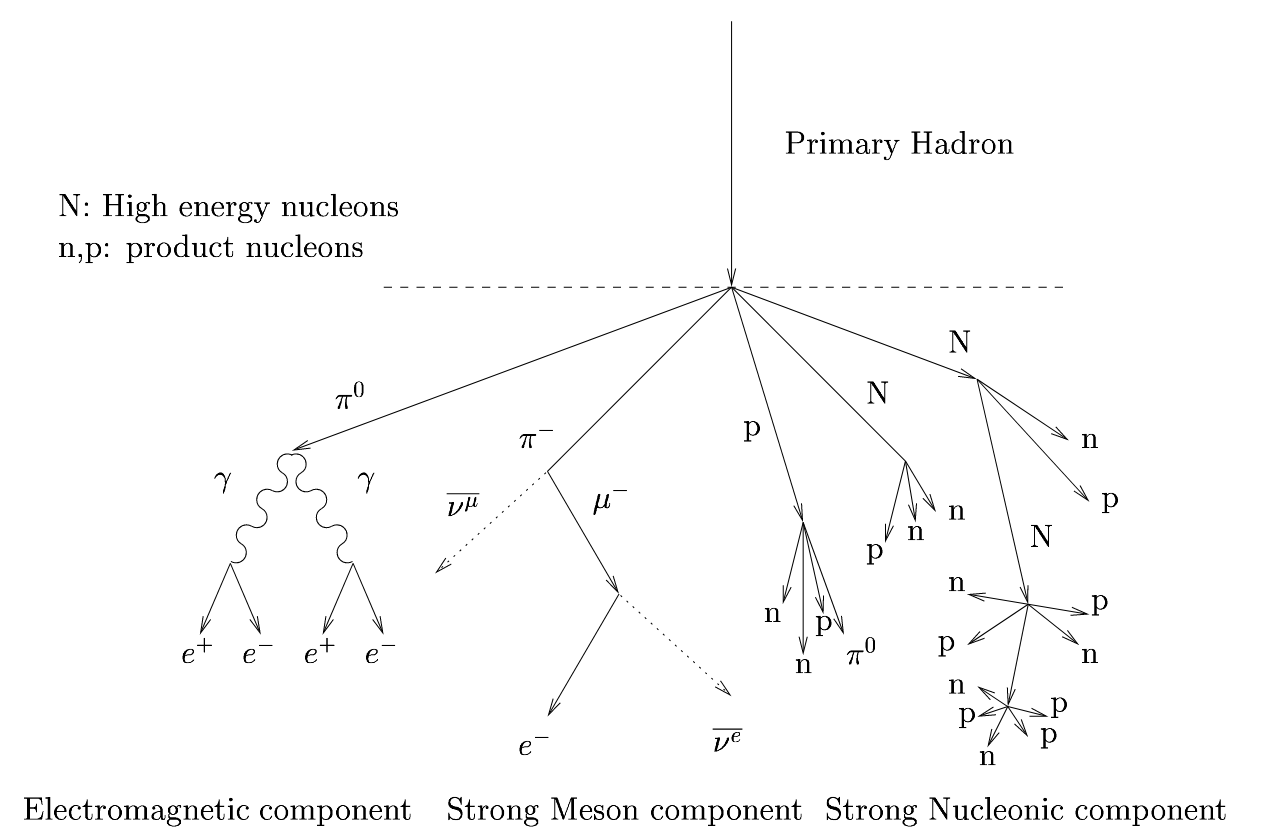
\includegraphics[width=\linewidth]{images/hadron_shower_illustration.png}
	\end{subfigure}%
	\begin{subfigure}{.2\textwidth}
 		\centering
		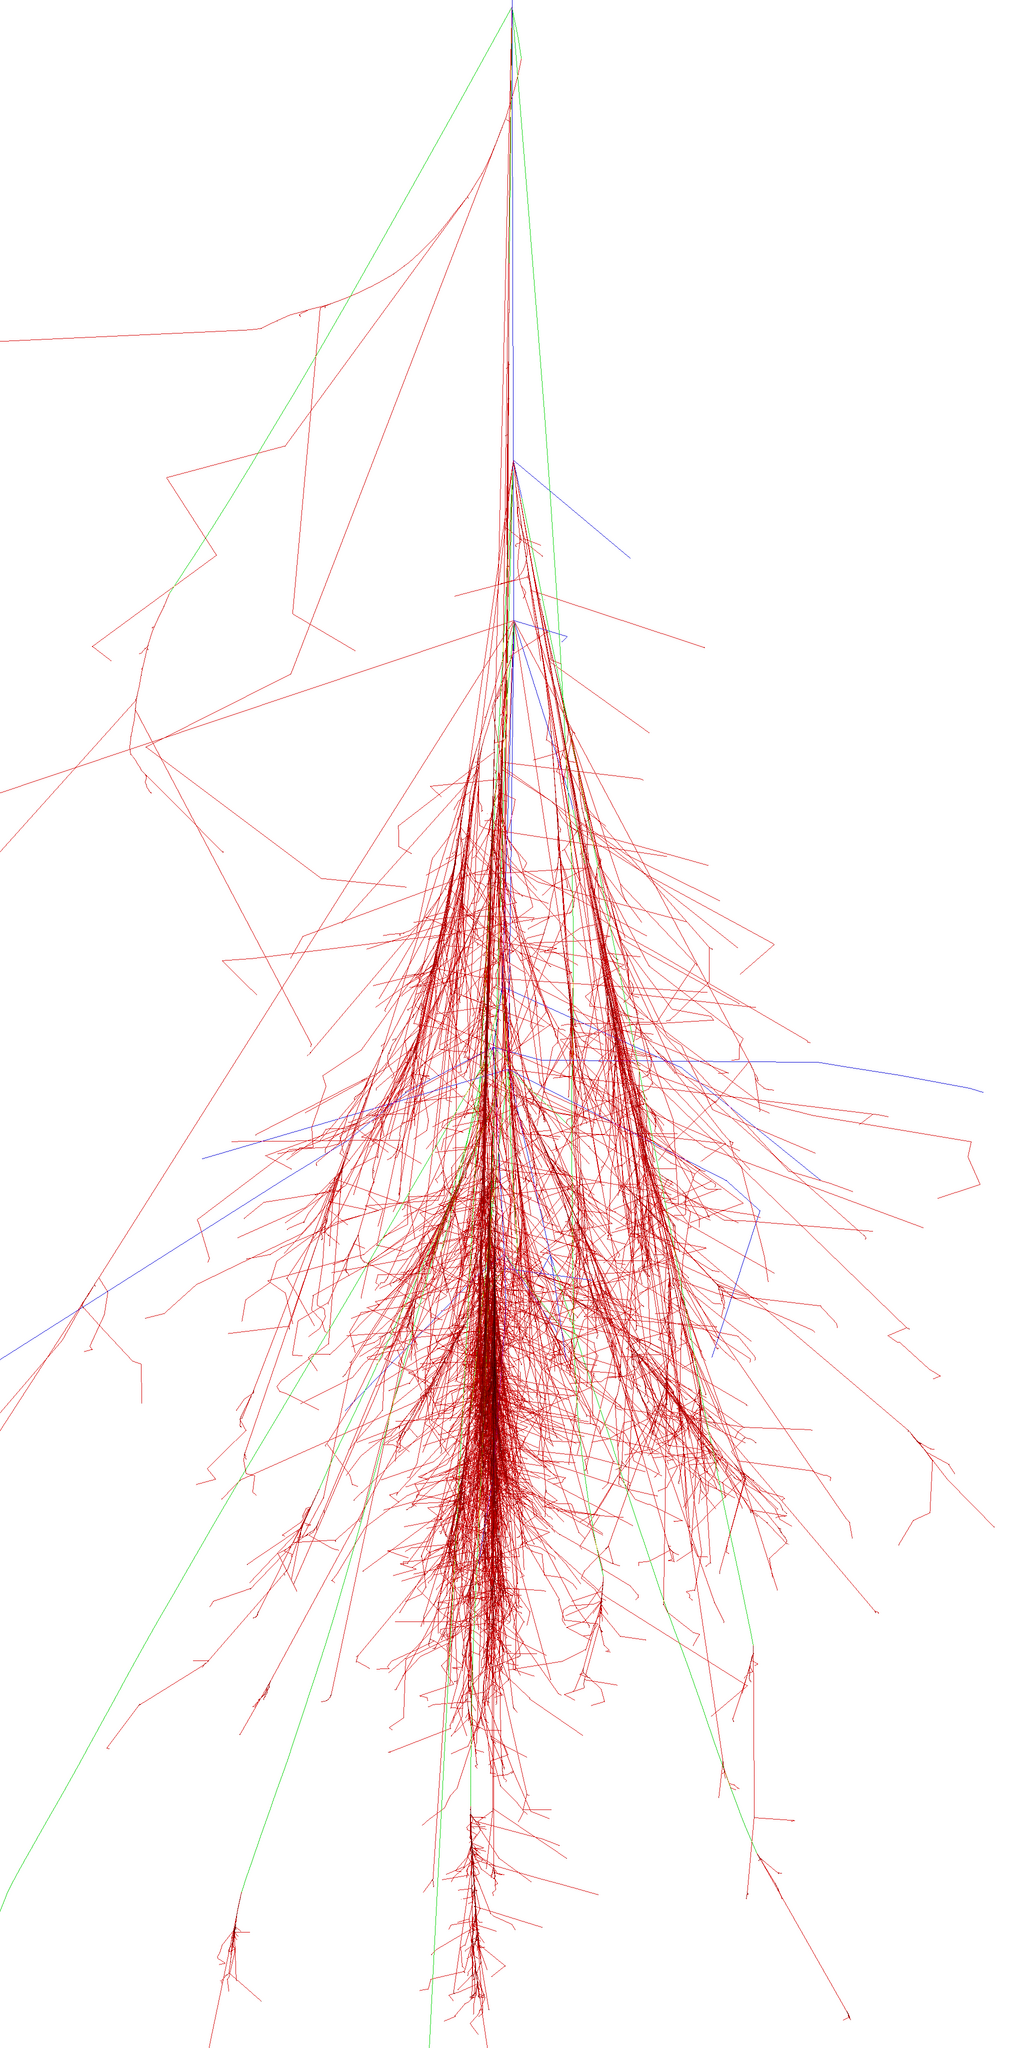
\includegraphics[width=\linewidth]{images/corsika_100gev_proton.png}
	\end{subfigure}
	\caption{Schematic illustration and simulation of a proton air shower.\\
		Left: A purely qualitative,
		schematic illustration of the generation of a hadronic shower.
		It shows how the primary hadron generates different subshowers
		with vastly different particles.
		The image is taken from an inaugural thesis 
		by Stefan Funk \cite{funk_doctor}.\\
		Right: A \SI{100}{\giga\electronvolt} proton-shower as xz-projection,
		simulated with CORSIKA.
		The shower is less contained than the gamma shower of equal energy in 
		figure \ref{fig:gamma_shower}.
		Different colors indicate different particle types.
		The image is taken from 
		the CORSIKA-website \cite{corsika_showers}.}
	\label{fig:proton_shower}
\end{figure}

\subsection{Measuring Events}
\label{sec:measuring}

The way IACTs detect particle showers in the atmosphere is by their emittance 
of Cherenkov light. Cherenkov light gets emitted whenever a 
charged particle moves through a dielectric medium with a velocity 
exceeding the local speed of light, which happens in air for the
highly relativistic particles we are lokking at.

Cherenkov photons get collected by the mirror(s) of a telescope
and projected onto a camera system mounted above the mirror.
With this setup IACTs usually reach a field of view of a few degree.
Figure \ref{fig:iact_mirror_camera} illustrates this setup.

\begin{figure}
	\centering
	\captionsetup{width=0.9\linewidth}
	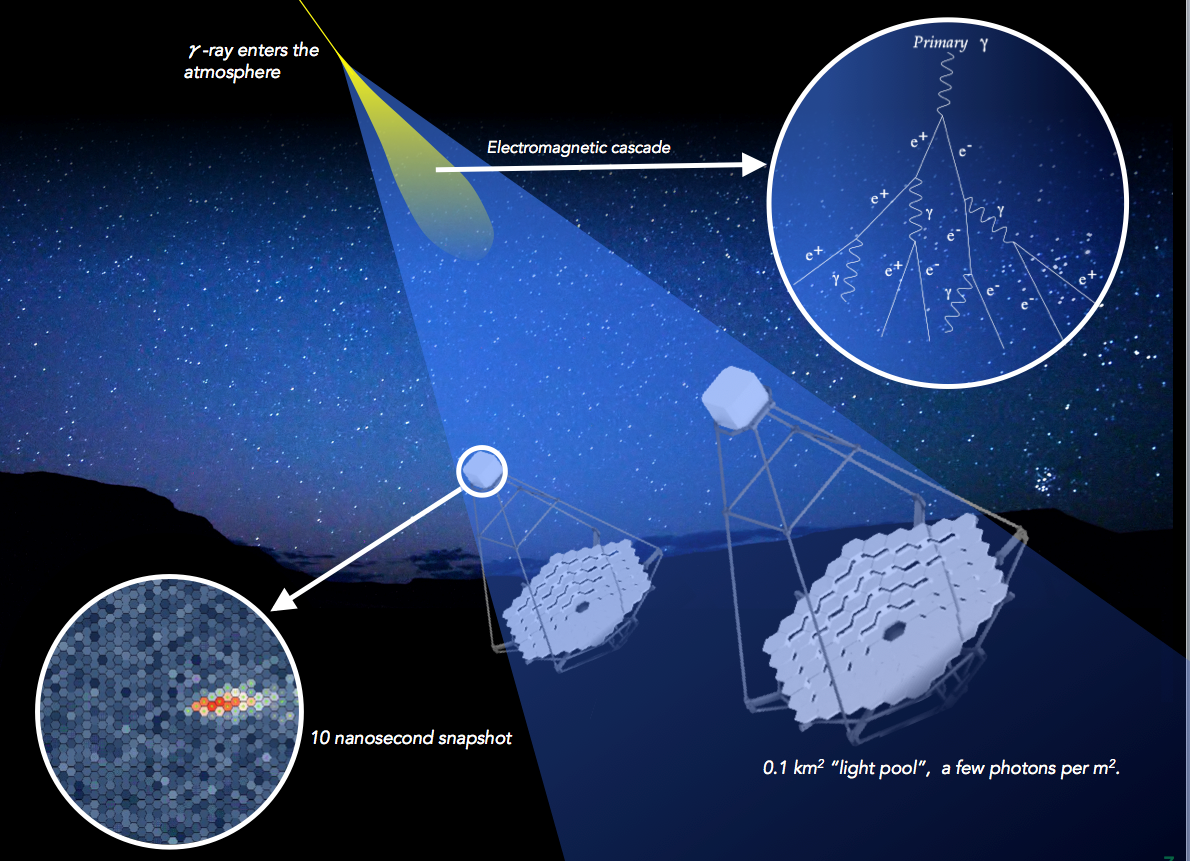
\includegraphics[width=0.9\textwidth]{images/cta47.png}
	\caption{A schematic illustration of the working principles of 
	an IACT experiment:
	A $\gamma$-ray produces an air shower in the atmosphere
	that points roughly towards the telescopes.
	Cherenkov light from the air shower 
	hits the mirrors and gets focused into a camera mounted on top.
	An illustration of the resulting image after integrating 
	\SI{10}{\nano\second} of the pixel measurements
	can be seen in the left bottom corner.
	The image is taken from the official CTA-website \cite{cta_web}.}
	\label{fig:iact_mirror_camera}
\end{figure}


Upon detection of a shower and performing the low-level analysis,
the usual tasks of a high-level analysis include reconstructing 
three key properties of the primary particle:
\begin{enumerate}
	\item{Shower type (e.g. gamma or hadronic)}
	\item{Primary particle energy}
	\item{Shower direction/source position}
\end{enumerate}

In most cases the reconstruction can be improved heavily by cleaning the image first.
Figure \ref{fig:shower_cleaning} shows a simulated $\gamma$-induced shower image
in the camera of the Large Sized Telescope (LST, see section \ref{sec:lst} for more details of the telescope)
before and after cleaning.

\begin{figure}
	\centering
	\captionsetup{width=0.9\linewidth}
	\begin{subfigure}{.45\textwidth}
  		\centering
  		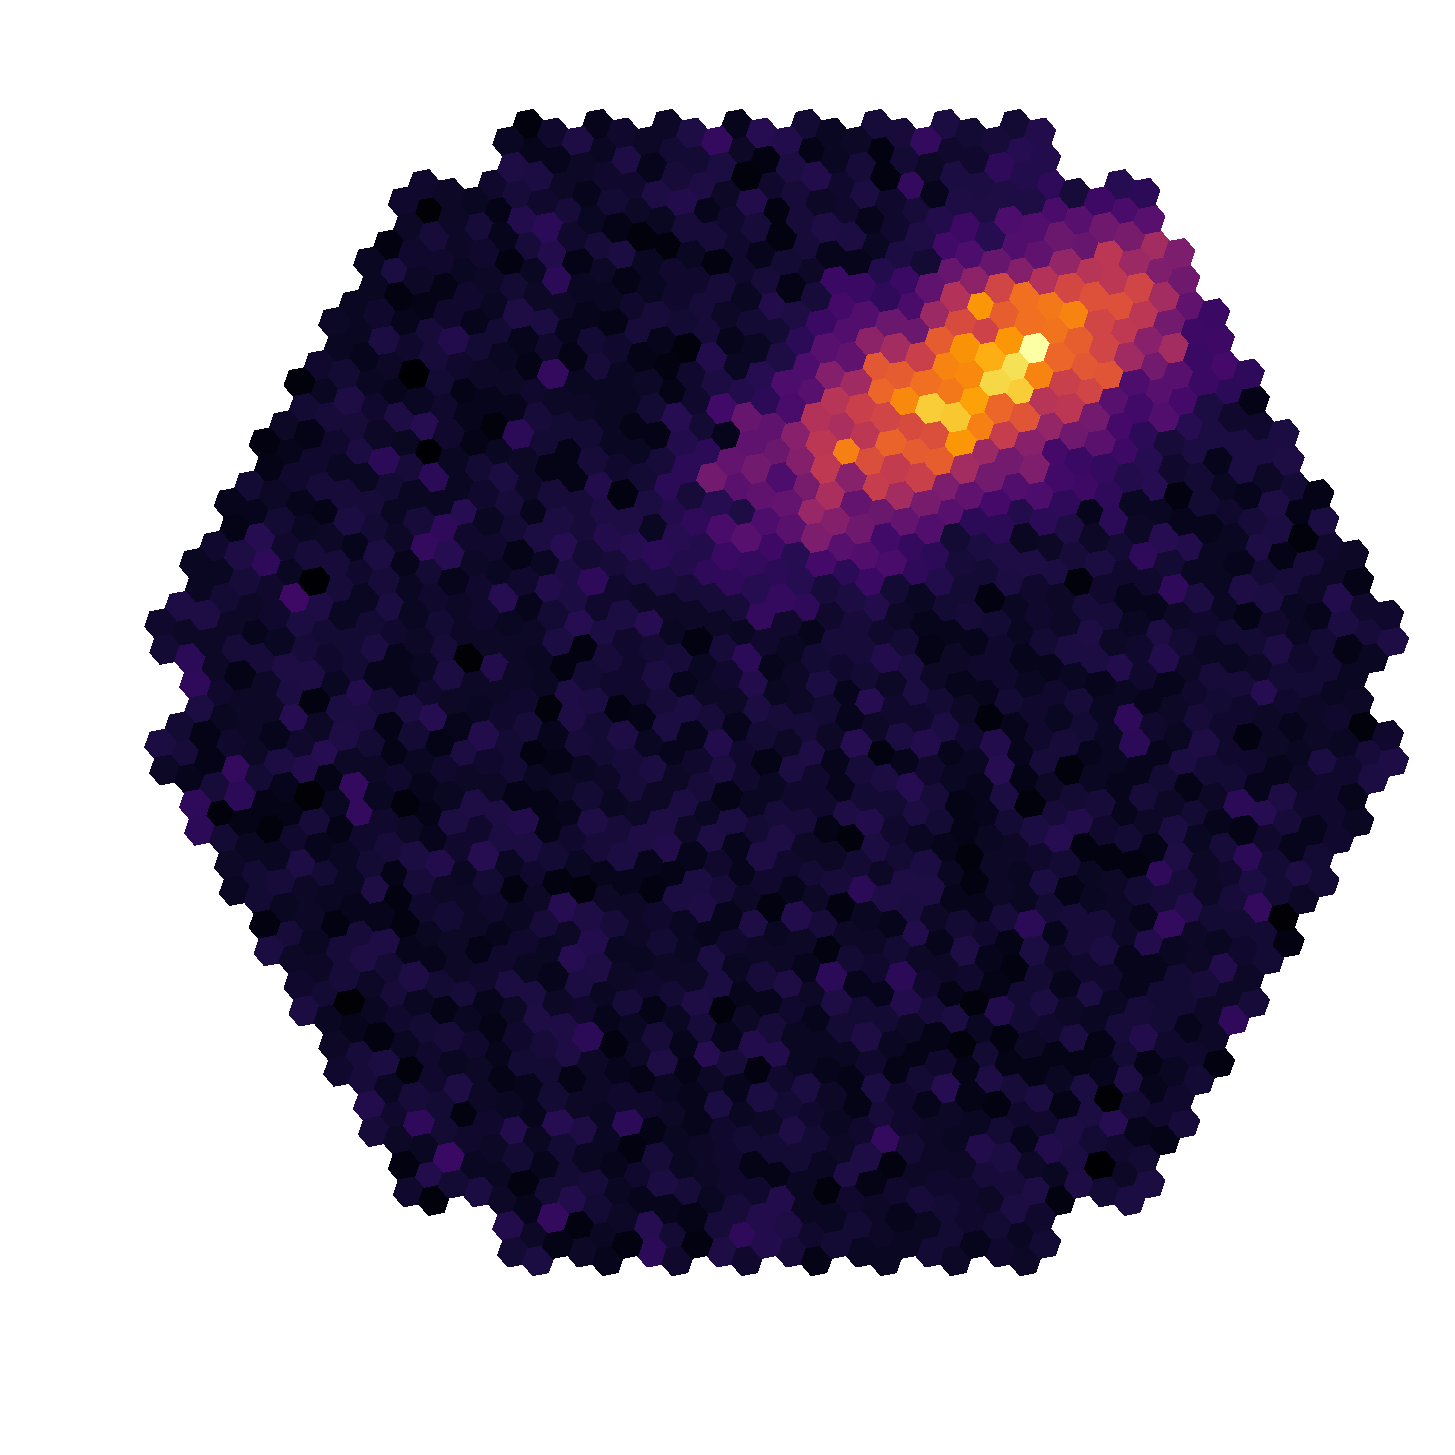
\includegraphics[width=\linewidth]{Plots/hillas_raw.pdf}
	\end{subfigure}%
	\begin{subfigure}{.45\textwidth}
 		\centering
		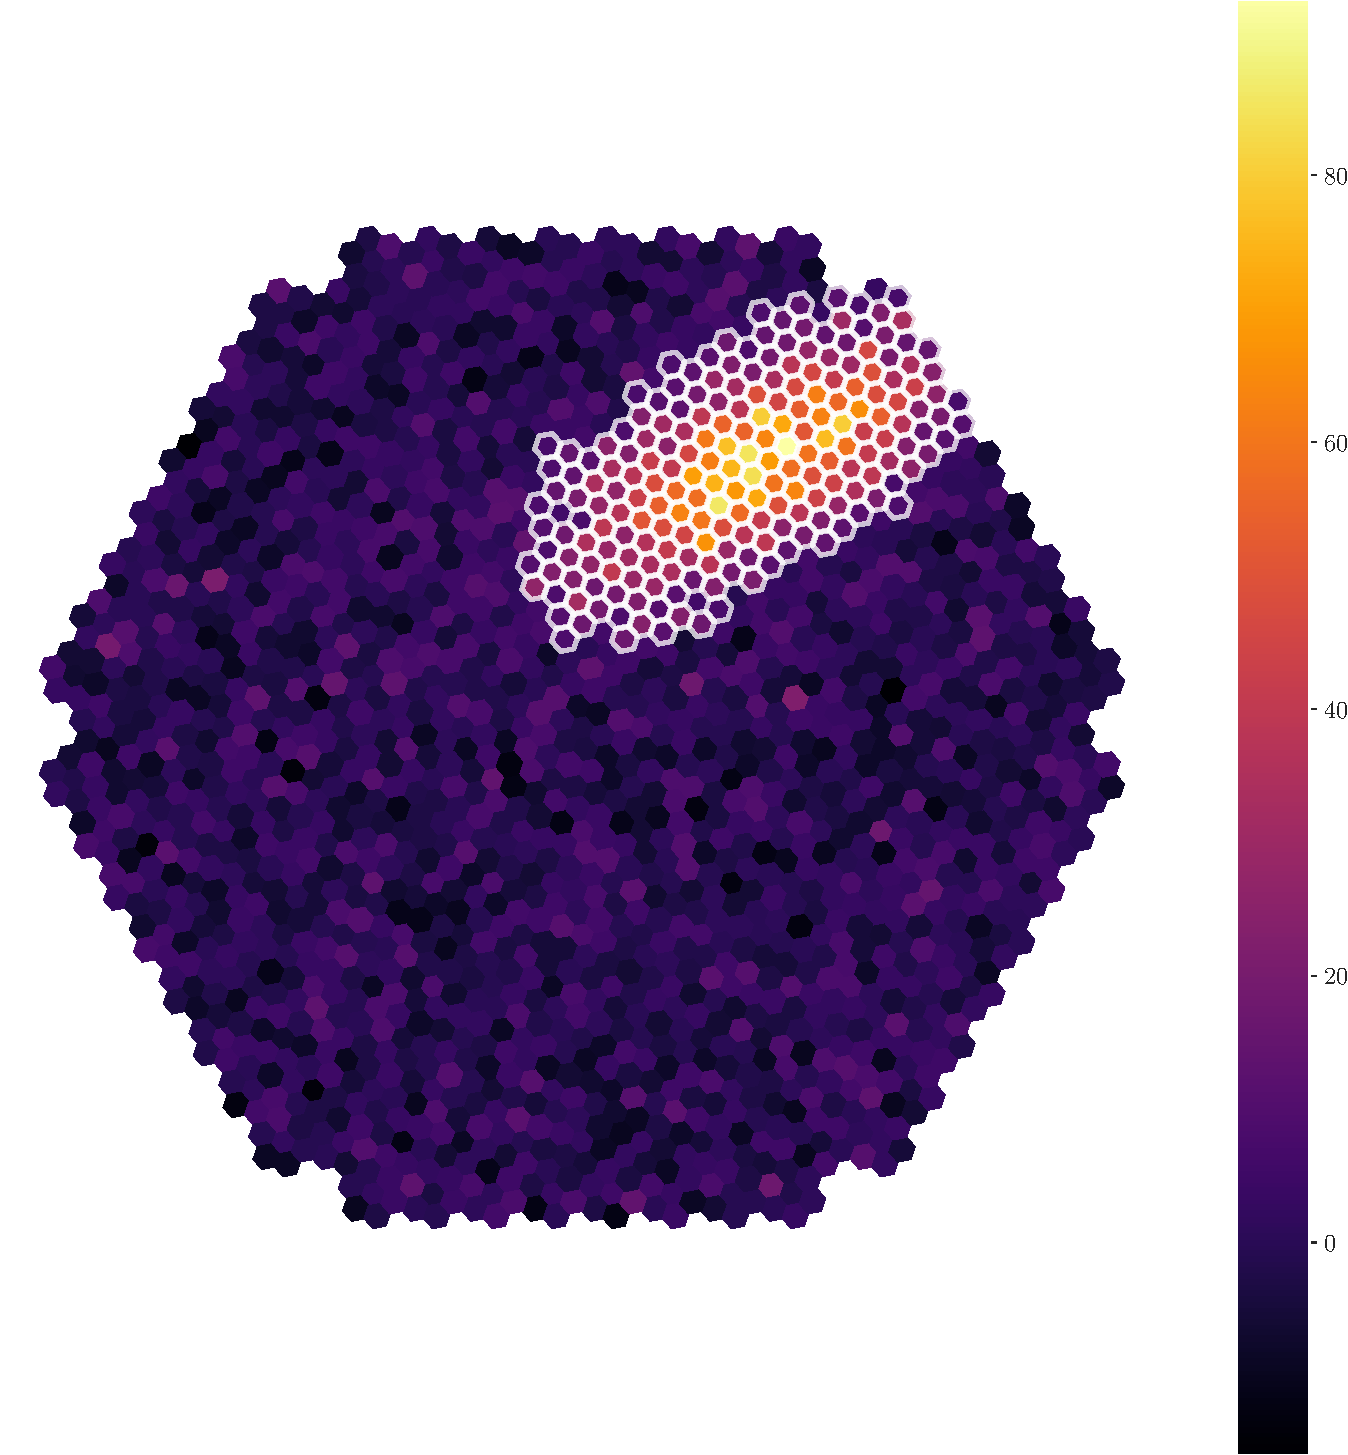
\includegraphics[width=\linewidth]{Plots/hillas_cleaned.pdf}
	\end{subfigure}
	\caption{An idealized gamma-shower in the camera of a LST
	    before and after cleaning.
		The pixel colors show the intensity as integrated 
		waveform in each pixel. 
		Brighter color indicates higher intensity.\\
		Left: The signal directly after
		the waveform integration. Non-signal pixels are noisy. 
		Right: Image after the cleaning-algorithm has been 
		applied. The noise in the non-signal pixels is gone,
		improving the analysis.}
	\label{fig:shower_cleaning}
\end{figure}

The analysis then usually involves describing the 
shower image as an ellipse and calculating the so called hillas parameters,
allowing the description of the shower image with only a handful of parameters.
The historical approach can be read up in 
a famous paper of A.M. Hillas \cite{hillas_params}.

An illustration with the hillas ellipse on top of the shower image 
can be seen in figure \ref{fig:hillas_params}.
This also includes an estimate of the true source position with the DISP-method
which we will use and explain at later stages.

\begin{figure}
	\centering	
	\captionsetup{width=0.9\linewidth}
	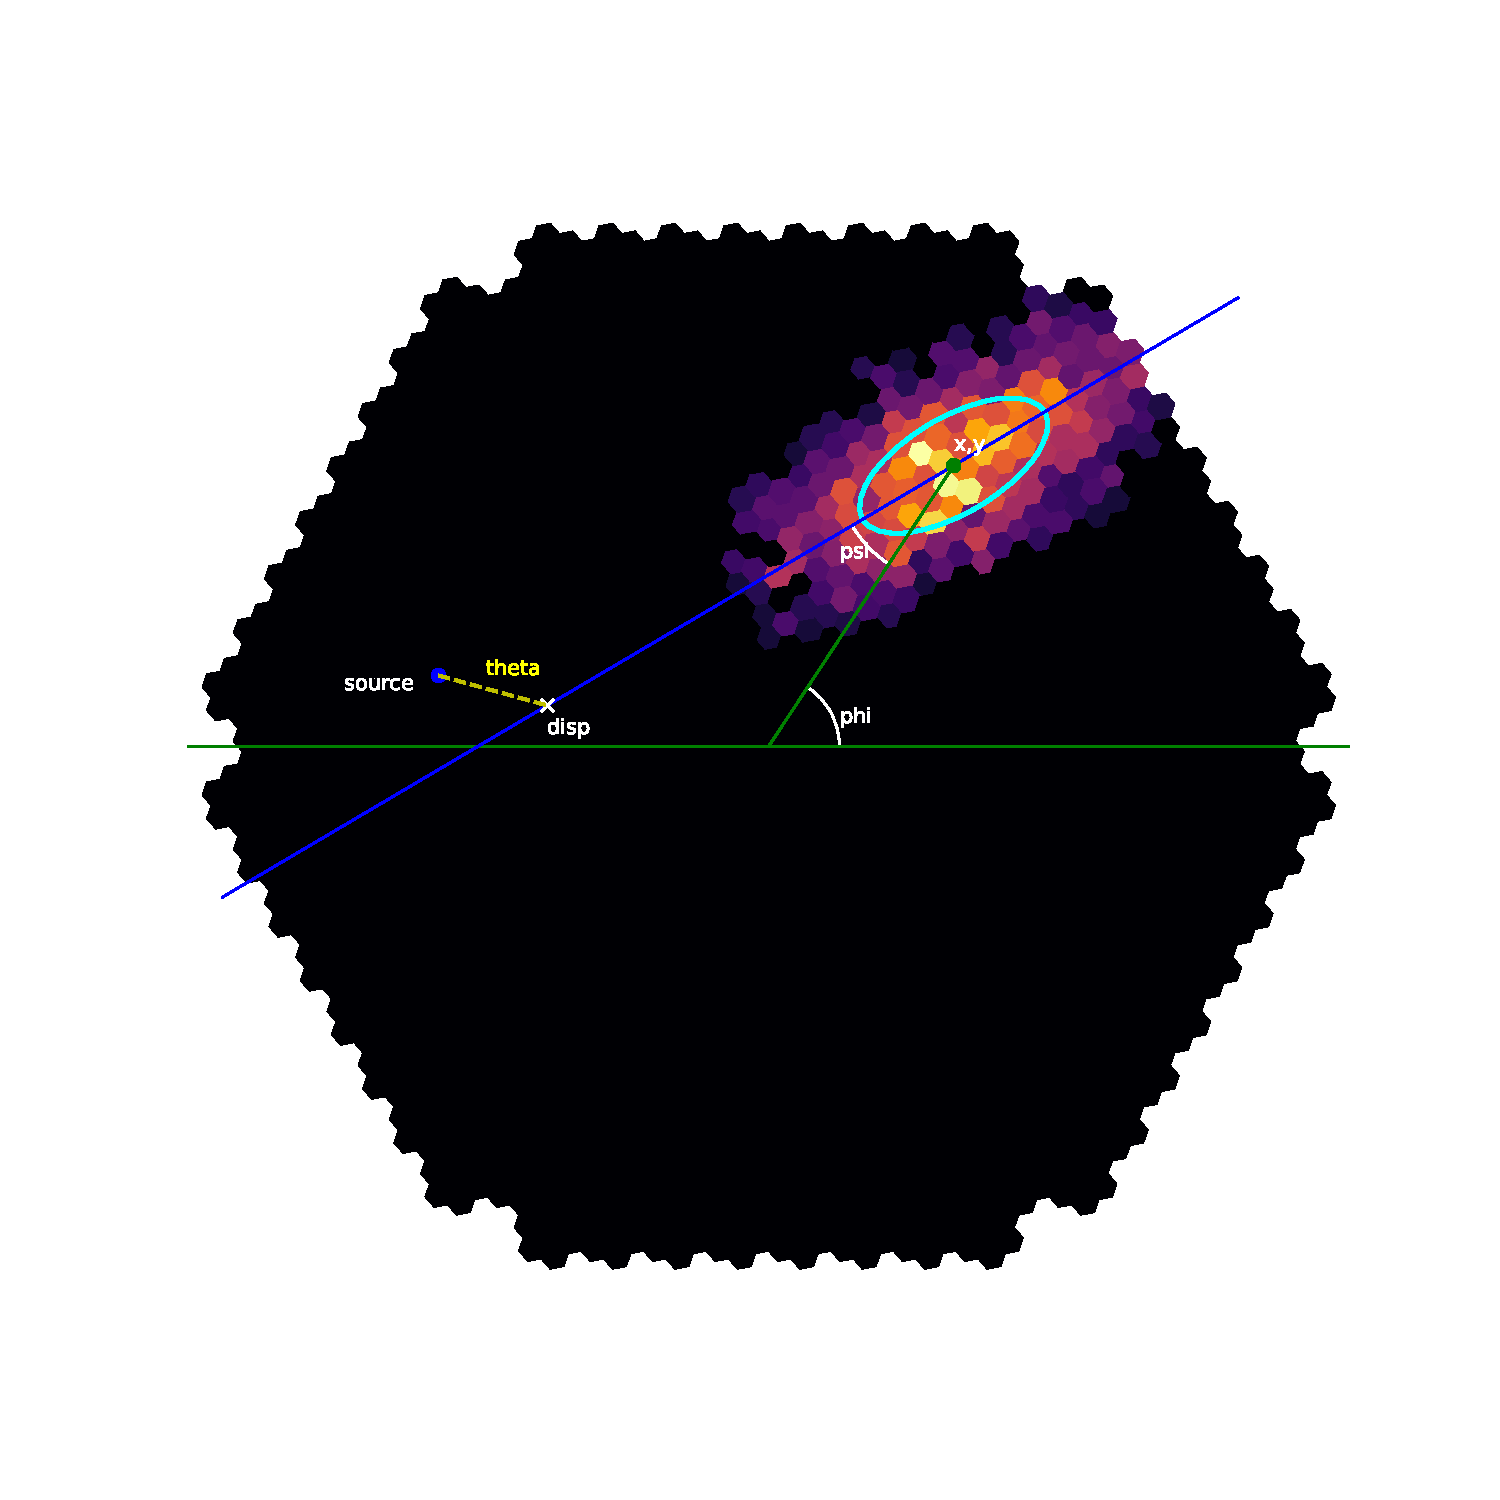
\includegraphics[width=.6\textwidth]{Plots/hillas_complete.pdf}
	\caption{The same cleaned shower-image as in figure \ref{fig:shower_cleaning}
	with the hillas-parameters calculated and marked in the camera frame.
	The parameters $\phi$, $\psi$, $x$ and $y$ describe the 
	orientation and position of the shower ellipse in the camera frame.
	The shower axis constrains the possible source position. 
	Applying the DISP-method two possible points remain.}
	\label{fig:hillas_params}
\end{figure}

With the hillas parameters calculated, the reconstruction of the 
primary particles properties can be done:

The primary \textbf{particle energy} is mostly described by the contained light in the image combined with 
an estimate of how much of the light missed the camera. 

The \textbf{particle type} can be reconstructed 
by looking at the image shape.
As we saw earlier, $\gamma$ and hadronic showers have different properties, 
resulting in different images. The assumption of a single, elliptic signal
area only works reasonably well for $\gamma$-showers.
A representation of different shower types can be seen in figure \ref{fig:compare_showers}.

\begin{figure}
	\centering
	\captionsetup{width=0.9\linewidth}
	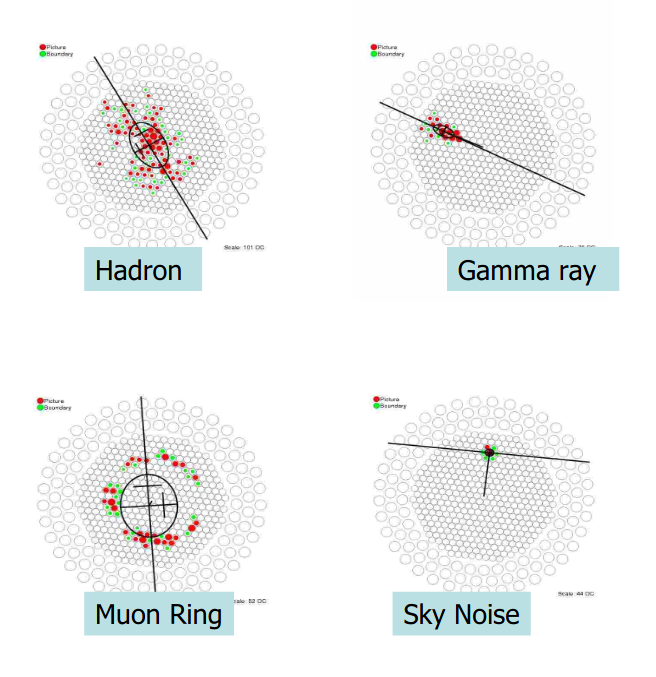
\includegraphics[width=.9\textwidth]{images/shower_types.png}
	\caption{A comparison of different shower types as seen 
	by the Whipple telescope.
	Hadronic showers are more separated than gamma showers and tend to
	form multiple clusters in the camera.
	Muons often times produce ring-like images in the camera (WHY?).
	The image is taken from an introduction lecture by Albrecht Karle \cite{icecube_showers}.}
	\label{fig:compare_showers}
\end{figure}

For the reconstruction of the \textbf{source position}
one possible way involves using the DISP-method in some way.

As basic estimation one can predict the shower origin by 
transforming the center of gravity (cog) of the image onto the sky plane.
The DISP-method assumes that the 
center of gravity is displaced relative to the
real source position depending on the angle the photon arrived at the telescope.
With higher angles the shower ellipse gets more eccentric as well.
The ellipsicity of the ellipse is thus a measure for the displacement of the true 
source position.
If one assumes the true source position to be on the main shower axis of the ellipse,
finding this position simplifies to finding a single point on the main shower axis.

Monoscopic experiments, that make use of the DISP method, need to resolve the head-tail-ambiguity:
Knowing the distance from the cog leaves two possible points, one on either side 
of the ellipse.
Stereoscopic experiments can resolve this ambiguity by combining the images from 
multiple telescopes, as can be seen in figure \ref{fig:stereo_shower}.

\begin{figure}
	\centering
	\captionsetup{width=0.9\linewidth}
	\hspace*{0.1\textwidth}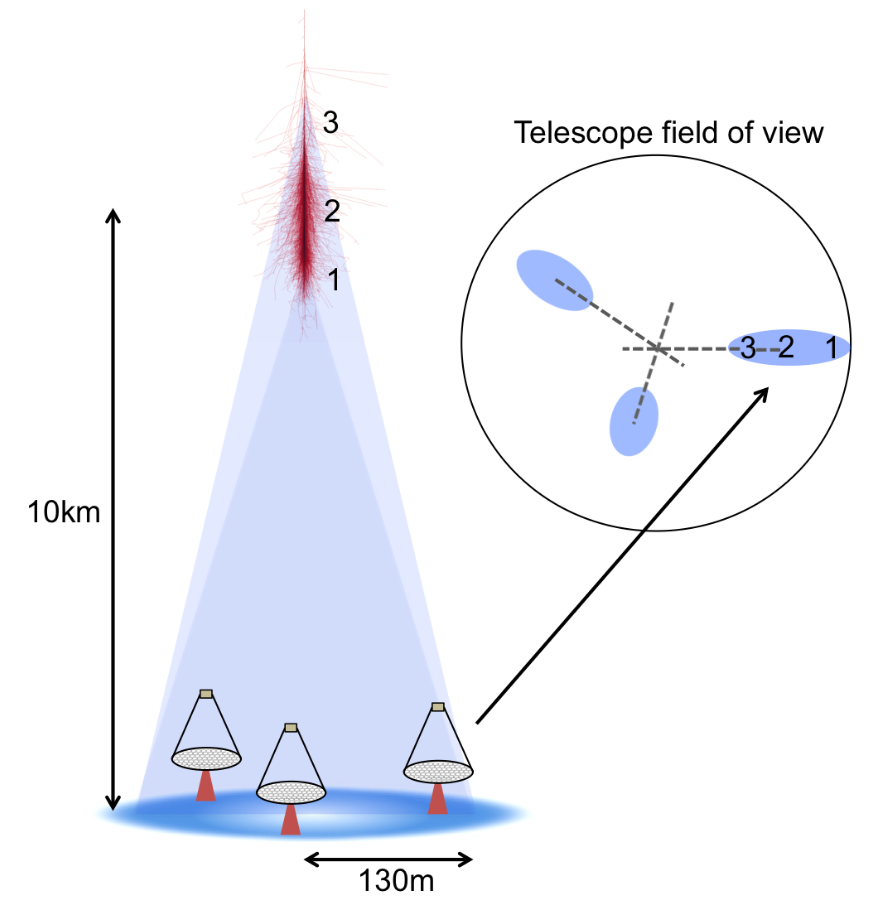
\includegraphics[width=0.9\textwidth]{images/stereo_shower.png}
	\caption{An illustration of an air shower captured with multiple telescopes.
		Each telescope captures an elliptic image.
		The image axes get intersected to reconstruct the arrival direction
		of the primary particle.
	    The image is taken from \cite{2015arXiv151005675H}.}
	\label{fig:stereo_shower}
\end{figure}


